\newpage
\section{Literature Review}
% \textit{What is the problem to be solved, and it's significance?
% \begin{itemize}
%     \item Brief background to project
%     \item Summary of literature relevant to project
%     \item Identification of "gaps" in the literature
% \end{itemize}}

% The literature review is not just about presenting descriptions of the important papers you have found, but telling a meaningful story and, where appropriate, some critical discussion of previous findings (i.e. was another study useful but flawed?). Remember that you may read hundreds of papers/books/web pages etc., but often only about 20 or 30 are really important, and these are the ones you will mention in your literature review, which this report will be a concise version of. This section needs to flow logically, and this does not always imply that the material is chronological. By the end, the reader should have a clear appreciation of what the major work in the field was, why it is relevant to the current project, and where the unknowns and questions lie (\textbf{research gaps}) – these are the issues that you are going to address with your thesis research.

% For the purposes of this report, this section will be \textbf{12-15 pages long}. Remember to reference properly any material that you obtain from literature or other sources. If you are unsure how to discuss literature properly, find a really good review paper on your topic, or if there isn’t one, a similar topic, and you will have a good example to refer to.

\subsection{Principles of Photovoltaic Modules}
\subsubsection{What are photovoltaic modules?}
Photovoltaic modules, commonly known as solar panels, are devices that convert sunlight into electrical energy. \cite{EnelGreenPower2025PhotovoltaicModule}\cite{U.S.DEPARTMENTofENERGY2025SolarBasicsb}\vspace{0.5em}

\subsubsection{What is the photoelectric effect?}
Sunlight is made up of massless particles called photons, which possess a certain amount of energy. When these photons strike the surface, they knock electrons off of it, known as photoelectrons. This is known as the photoelectric effect, shown in Figure \ref{fig:photoelectric_effect_diagram}.\vspace{0.5em}

\begin{figure}[ht]
    \centering
    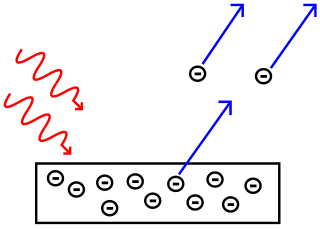
\includegraphics[width=0.4\textwidth]{Figures/photoelectric_effect_diagram.png}
    \caption{Photoelectric Effect Diagram \cite{KhanAcademy2025PhotoelectricEffect}}
    \label{fig:photoelectric_effect_diagram}
\end{figure}
\FloatBarrier

\noindent The photoelectric effect will occur only if the frequency of the radiation is greater than the threshold frequency of the metal. The threshold frequency is the minimum frequency of light that causes electrons to be emitted from a material. The proportional relationship that exists between the threshold frequency and the work function is shown in Equation \ref{eq:workfunction} below:
\begin{equation}
    E = hf_0
    \label{eq:workfunction}
\end{equation}
Where:
\begin{itemize}
    \item $E$ is the work function.
    \item ($h = 6.62607015 \times 10^{34}$ joule-second) is Planck's constant.
    \item $f_0$ is the threshold frequency. 
\end{itemize}\vspace{0.5em}
\noindent The work function refers to the minimum amount of energy needed to remove an electron from a metal surface. If photons with enough energy hit the surface, they can transfer their energy to the electrons allowing them to escape. If the energy of the incident photons is less than the work function, no electrons will be emitted, regardless of the intensity of the light. \cite{ScienceABC2025PhotoelectricBeginners}\vspace{0.5em}

\subsubsection{How do photovoltaic modules work?}
A photovoltaic module is made up of multiple photovoltaic cells, commonly known as solar cells. Each photovoltaic cell is made of semiconductor material, which is placed between the conductive layers. The most common semiconductor material used to make photovoltaic cells is silicon, accounting for 95 percent of photovoltaic modules sold worldwide. \cite{U.S.DEPARTMENTofENERGY2025SolarBasics} These photovoltaic cells use the photovoltaic effect to convert solar energy into electrical energy.\vspace{0.5em}

\noindent As shown in Figure \ref{fig:photovoltaic_cell_diagram}, a silicon photovoltaic cell is composed of two different layers of silicon: an n-type silicon layer, which has additional electrons, and a p-type silicon layer, which has extra spaces for the electrons, called holes.\par

\noindent ADD IN THE STUFF ABOUT DOPING (CAN BE FOUND IN BARRY'S SECOND PARAGRAPH IN 2.1.)

\begin{figure}[ht]
    \centering
    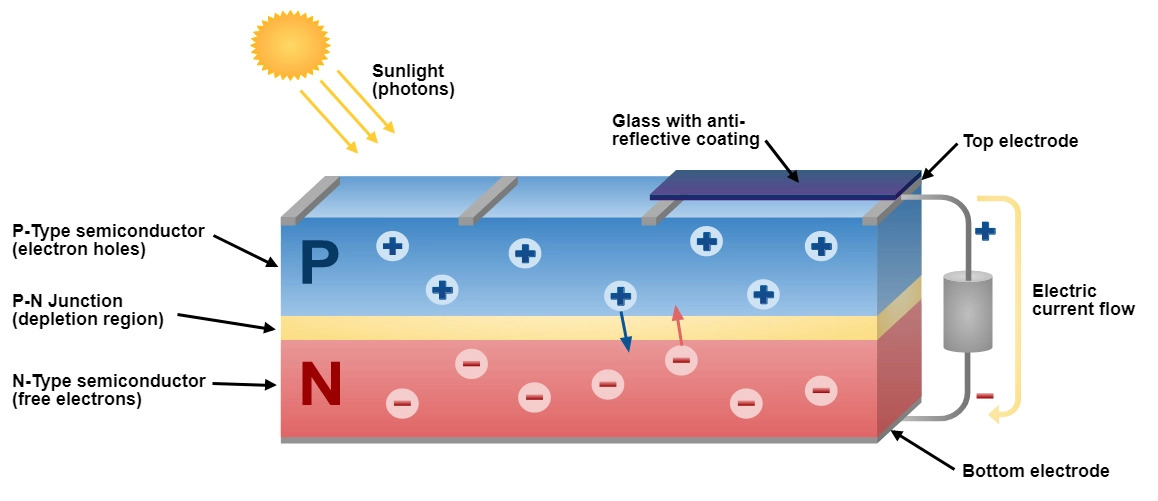
\includegraphics[width=1\textwidth]{Figures/photovoltaic_cell_diagram.jpg}
    \caption{Photovoltaic Cell Structure Diagram \cite{Gupta2020SolarVehicle}}
    \label{fig:photovoltaic_cell_diagram}
\end{figure}
\FloatBarrier

\noindent When a proton strikes the silicon photovoltaic cell with the required energy, an electron is knocked out of its bond. Because of the electric field at the p-n junction, the negatively charged electron moves toward the n-side, while the resulting positively charged hole is attracted to the p-side. The free electrons are collected by thin metal fingers positioned at the top of the photovoltaic cell, before travelling through an external circuit. After electrical work is performed, the electrons are returned to the conductive aluminium sheet positioned at the back of the photovoltaic cell. Since electrons follow a continuous cycle and are the only moving components, there is no wear and tear, allowing photovoltaic cells to last for decades. \cite{TED-Ed2025HowKomp} However, they still have limitations.\vspace{0.5em}

\subsection{Limitations of Photovoltaic Modules}
\subsubsection{What are the limitations of Photovoltaic Modules?}
- A significant limitation of photovoltaic modules is their electrical efficiency.\par
\noindent- A standard photovoltaic module typically converts between 6 and 20 percent of incoming solar radiation into electrical energy.\par
\noindent - The remaining 80 to 94 percent of incident solar radiation is primarily converted into heat, raising the temperature of the photovoltaic module and subsequently reducing its energy conversion efficiency. \cite{Dubey2013TemperatureReview}\par\vspace{1em}

\noindent - A 2010 study led by H.G. Teo from the National University of Singapore further refined the electrical efficiency range of photovoltaic modules to between 8 and 14 percent.\par
\noindent \textbf{What did Teo et al. aim to do in this paper?}\par
\noindent - Teo et al. \cite{Teo2012AnModules} focused on the comparing the electrical efficiency of the photovoltaic module with and without cooling.\par
\noindent \textbf{What did he find out? Did he achieve his goals/aims?}\par
\noindent 
\noindent - Teo et al. \cite{Teo2012AnModules} observed electrical efficiency as a linear function of photovoltaic module temperature, shown in Figure \ref{fig:electrical_efficiency_vs_temperature_pv_module}.\par
\noindent - An increase in the module temperature resulted in a decrease in the module's electrical efficiency.\par

\begin{figure}[ht]
    \centering
    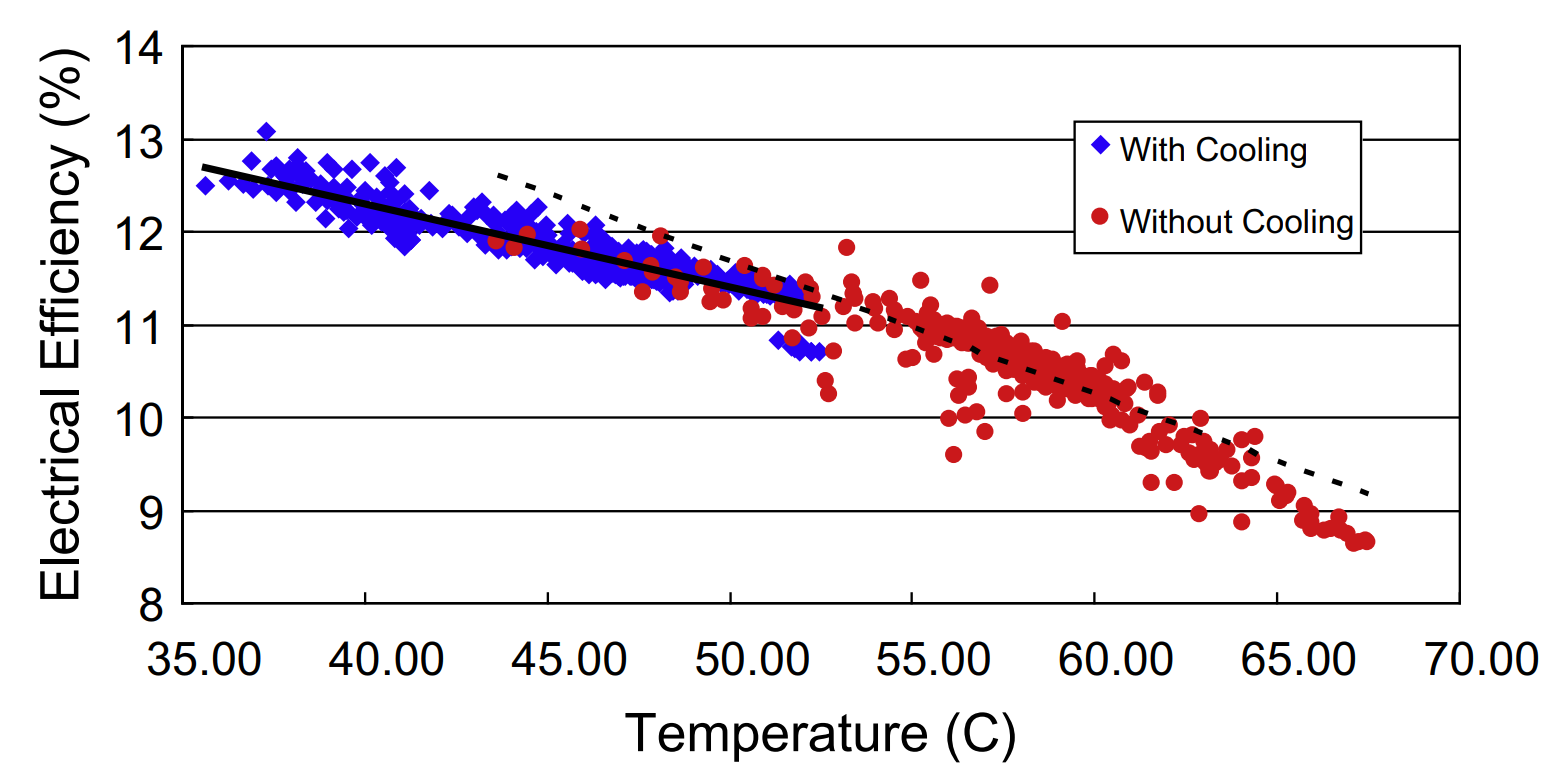
\includegraphics[width=0.75\textwidth]{Figures/electrical_efficiency_vs_temperature_pv_module.png}
    \caption{Electrical efficiency as a function of PV temperature \cite{Teo2012AnModules}}
    \label{fig:electrical_efficiency_vs_temperature_pv_module}
\end{figure}
\FloatBarrier

\noindent - Teo et al.'s \cite{Teo2012AnModules} experiment considered cooling and non-cooling cases.\par
\noindent - In Figure \ref{fig:electrical_efficiency_vs_temperature_pv_module}, Teo et al. observed that without active cooling, the module temperature was much higher than when active cooling was introduced under the same meterological conditions.\par
\noindent - As a result, the presence of active cooling improved the electrical efficiency of the photovoltaic module from between 8 and 9 percent to between 12 and 14 percent.\vspace{1em}

\noindent WHAT WAS THE REASON!!! ** CARDI VOICE **\par
\noindent Key Words:\par
\begin{itemize}
    \item \texttt{[Bandgap]} What is the bandgap?
\end{itemize}


\subsubsection{How do we reduce the impact of these limitations?}
By finding ways to cool the module temperature.\par

\pagebreak
\subsection{Heat Transfer in Photovoltaic Modules}
% \subsection{Heat Transfer in Photovoltaic Modules}
% \begin{itemize}
%     \item What is heat transfer?
%     \item What are the types of heat transfer?
%     \item What is the fundamental concept of heat transfer?
%     \item What are some convection principles used to enhance heat transfer in a photovoltaic module?
% \end{itemize}

\subsubsection{Conduction} % How does conduction transfer heat in pv modules
\noindent What is conduction?\par
\noindent How can conduction be used to cool down photovoltaic modules?\par
\noindent Why are they not the optimal source of heat transfer for cooling down photovoltaic module?\par

\subsubsection{Radiation} % How does radiation transfer heat in pv modules
\noindent What is radiation?\par
\noindent How can radiation be used to cool down photovoltaic modules?\par
\noindent Why are they not the optimal source of heat transfer for cooling down photovoltaic module?\par

\subsubsection{Convection} % How does convection transfer heat in pv modules
\paragraph{Natural Convection and the Relevant Cooling Methods (Passive Cooling)} % What role does natural convection play in the convective heat transfer in pv modules
\paragraph{Forced Convection and the Relevant Cooling Methods (Active Cooling)} % What role does natural convection play in the convective heat transfer in pv modules
\subsubsection{Vortex Generators: Vortex Induced Heat Induction} % How are vortices used to induce heat induction

\pagebreak
\subsection{Experimental Techniques}
\subsubsection{Infrared Thermography}
\subsubsection{Thermocouple Sensors}
\subsubsection{Particle Image Velocimetry}

\pagebreak
\subsection{Literature Gap}

\pagebreak


% \subsubsection{Vortex Induced Heat Transfer}
% \begin{itemize}
%     \item What is a vortex?
%     \item How does a vortex/system of vortexes induce heat transfer?
%     \item Are there any drawbacks of vortex-induced heat transfer? If so, what are they?
% \end{itemize}

% \subsubsection{Conduction}
% \begin{itemize}
%     \item What is conduction?
%     \item How can conduction be used to enhance heat transfer?
%     \item What are some examples of this principle in practice?
%     \item What were the results of this practice?
%     \item Are there any drawbacks of conduction as a method to enhance heat transfer?
% \end{itemize}

% \subsubsection{Radiation}
% \begin{itemize}
%     \item What is radiation?
%     \item How can radiation be used to enhance heat transfer?
%     \item What are some examples of this principle in practice?
%     \item What were the results of this practice?
%     \item Are there any drawbacks of radiation as a method to enhance heat transfer?
% \end{itemize}

% \subsection{Convective Photovoltaic Module Cooling Methods}
% \begin{itemize}
%     \item What is convection?
%     \item What are some cooling methods for convective photovoltaic modules?
% \end{itemize}

% \subsubsection{Cooling through Natural Convection}
% \begin{itemize}
%     \item What is Natural Convection?
%     \item How is natural convection used as a cooling method for photovoltaic modules?
%     \item Are there drawbacks to natural convection as a cooling method for photovoltaic modules?
%     \item How does forced convection compare to natural convection as a cooling method for photovoltaic modules?
% \end{itemize}

% \subsubsection{Cooling through Forced Convection}
% \begin{itemize}
%     \item What is forced convection?
%     \item How is forced convection used as a cooling method for photovoltaic modules?
%     \begin{itemize}
%         \item DC Fan Experiment
%         \item Floating Photovoltaic Module Experiment
%     \end{itemize}
%     \item Are there drawbacks to forced convection as a cooling method for photovoltaic modules?
%     \item Air vs Water Cooling Experiment
%     \item Air Cooled Modified Photovoltaic Module Experiment
%     \item Single Fin vs Multiple Fin Experiment
% \end{itemize}

% \subsubsection{Cooling through Vortex Generators}
% \begin{itemize}
%     \item What is a vortex generator?
%     \item What is the purpose of vortex generators?
%     \item Examples of Vortex Generator Experiments in the Context of Photovoltaic Module Cooling
% \end{itemize}